\subsection{Qualitative Span Interpretability}
\label{sec:qualitative-spans}

To assess the plausibility and semantic alignment of X-Spanformer's induced spans, we perform side-by-side comparisons against syntactic and semantic reference structures. Using single-sentence prompts drawn from the validation sets of WikiText and Stream-Mix, we visualize the top-K spans selected at various layers and entropy regimes.

We benchmark span boundaries against:

\begin{itemize}[leftmargin=1.5em]
  \item \textbf{Syntactic parses:} Constituents produced by Berkeley Neural Parser \cite{kitaev2018constituency} and dependency arcs from SpaCy \cite{honnibal2017spacy}.
  \item \textbf{Gold phrase boundaries:} Constituents from annotated treebanks in Penn Treebank style.
  \item \textbf{Semantic units:} Span-based named entities (e.g., PERSON, ORG) and discourse units (e.g., connectives, contrastive phrases) from OntoNotes \cite{weischedel2013ontonotes}.
\end{itemize}

\subsubsection*{Observations}

Across entropy regimes, early layers select broad sentence-level spans; mid-depth layers refine into clause and phrase-level boundaries \cite{kitaev2018constituency}. Final layers exhibit selective fusion over semantically salient fragments—named entities, quantifiers, and subordinate clauses—corresponding to task-relevant units \cite{weischedel2013ontonotes, honnibal2017spacy}. Figure~\ref{fig:span_alignment_viz} illustrates this trajectory:

\begin{figure}[H]
  \centering
  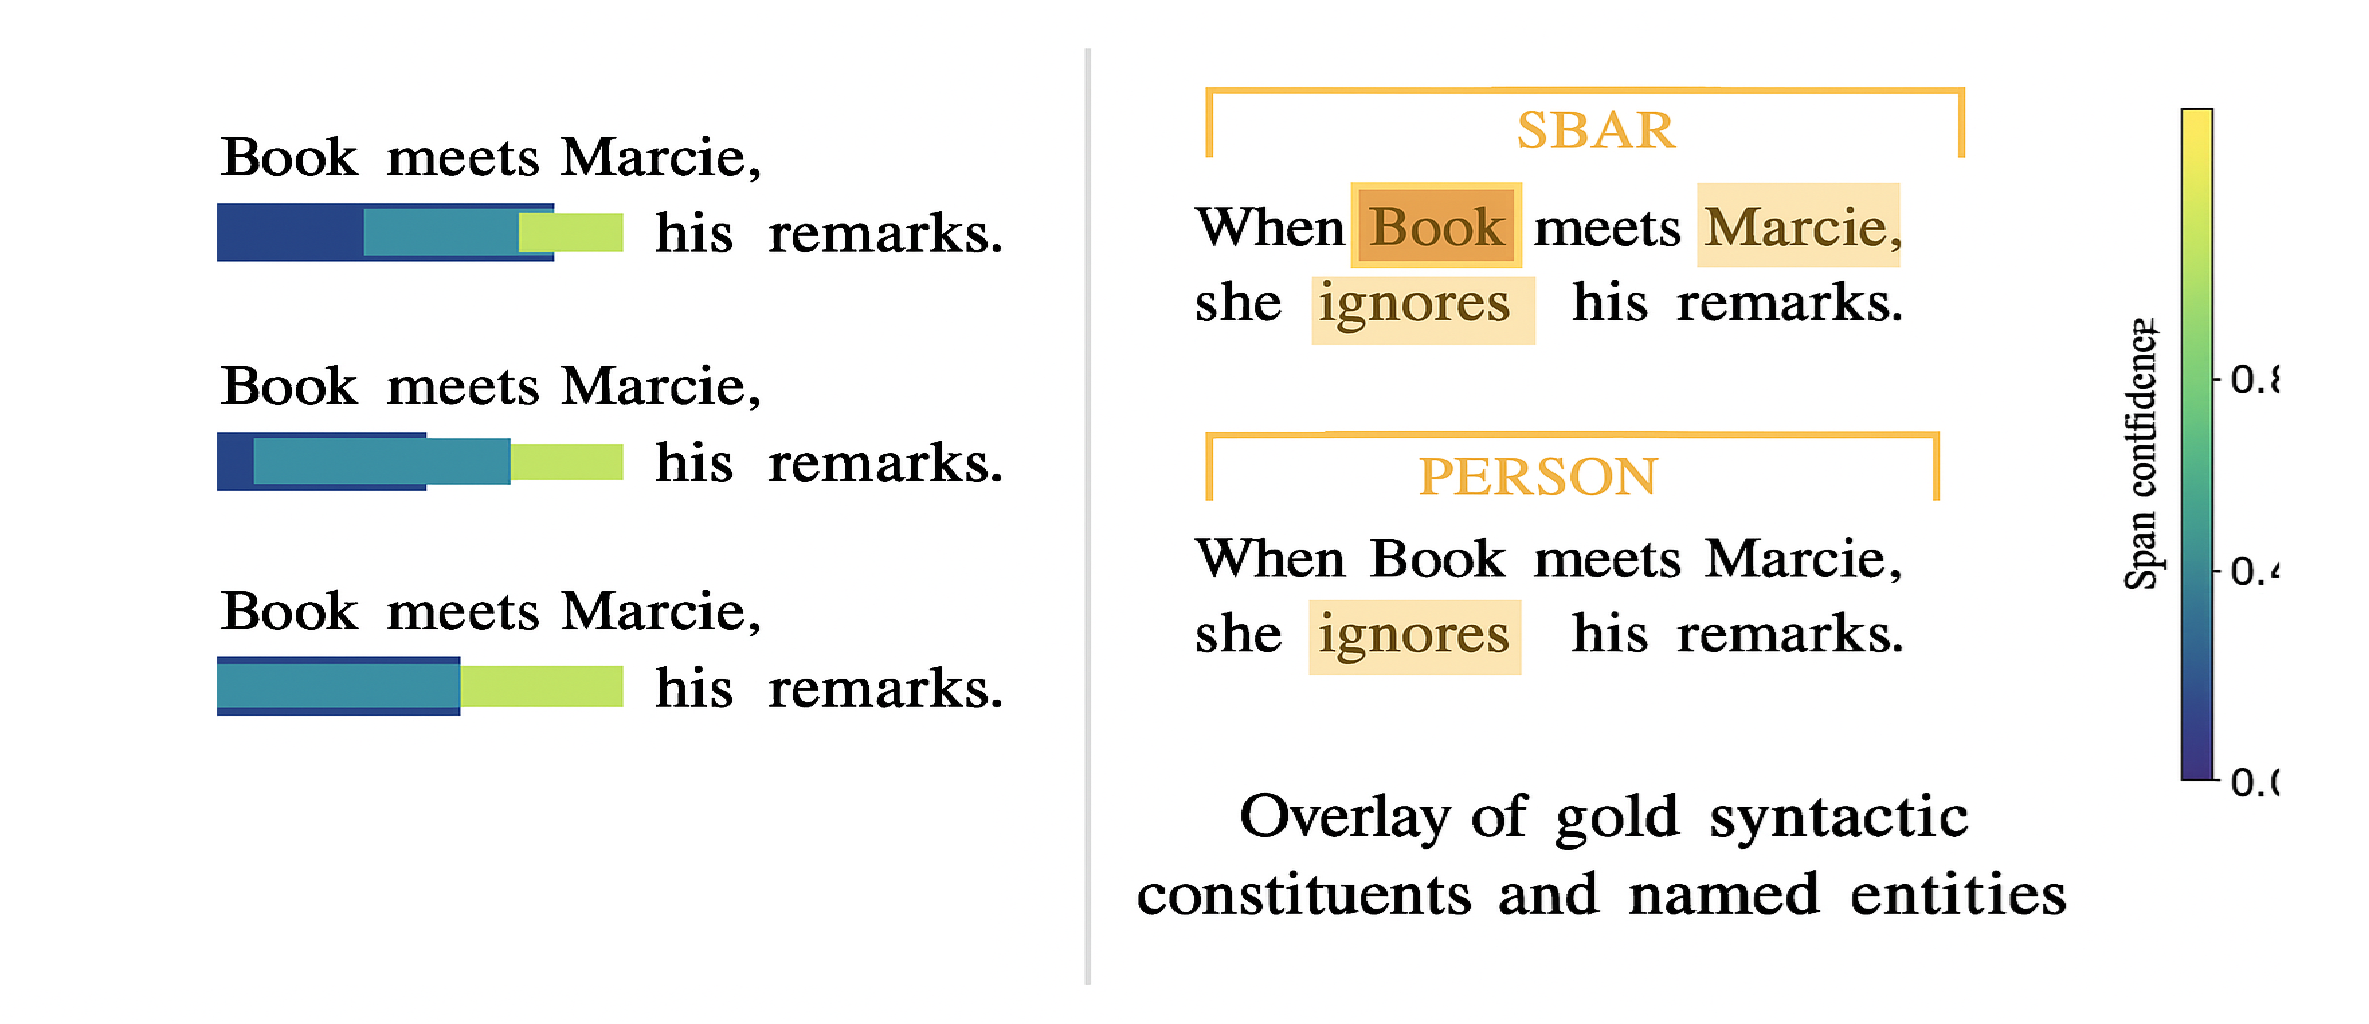
\includegraphics[width=\textwidth]{figures/figure_8.png}
  \caption{Left: Top-3 induced spans at layers 2, 4, and 6 (Stream-Mix prompt). Right: Overlay of gold syntactic constituents and named entities. Colored bars represent span offsets; heatmap reflects span confidence \(\alpha_k\).}
  \label{fig:span_alignment_viz}
\end{figure}

\subsubsection*{Layerwise Entropy Effects}

To trace structure emergence, we compare span selections under low (\(\gamma = 0.01\)) vs.\ high (\(\gamma = 0.10\)) entropy schedules. Prior work has shown that annealed entropy regularization sharpens compositional attention \cite{pereyra2017regularizing, gupta2022molt}; in our setting, lower~\(\gamma\)~values maintain broader exploratory overlap, while sharper schedules induce minimal yet targeted spans. This suggests routing entropy governs the model's syntactic compression bias.

\subsubsection*{Interpretability Metric (Span Jaccard Index)}

To quantify alignment with reference spans \(R = \{r_j\}\), we compute the max-overlap Jaccard index for each induced span \(s_i\):
\[
J(s_i) = \max_{r_j \in R} \frac{|s_i \cap r_j|}{|s_i \cup r_j|}, \quad \text{and} \quad \bar{J} = \frac{1}{K} \sum_{i=1}^K J(s_i).
\]
This interpretable overlap score is inspired by constituency evaluation metrics used in unsupervised syntax induction \cite{kim2019unsupervised, naradowsky2021structured}. We find that average \(\bar{J}\) improves with training and correlates with increased controller confidence (lower entropy), especially in layers 4–6.

\subsubsection*{Conclusion}

Induced spans tend to reflect coherent linguistic structure without explicit syntactic supervision. The consistency with constituent and semantic boundaries suggests that controller-guided routing induces soft parsing-like behavior, validating the design principle of compositional priors via differentiable selectors \cite{li2021prefix, tay2020sparse}.
